\documentclass[10pt,twocolumn]{article}

% use the oxycomps style file
\usepackage{oxycomps}
\usepackage{float}
\usepackage{biblatex}
\addbibresource{references.bib}

\pdfinfo{
    /Title (Comps Proposal)
    /Author (Oliver Wilkins)
}

% set the title and author information
\title{Comps Proposal}
\author{Oliver Wilkins}
\affiliation{Occidental College}
\email{wilkins@oxy.edu}

\begin{document}

\maketitle

\section{Problem Context}
The standard economic theory which has dominated the field over the past century is once which derived from a realization in the early 1900s that consumer choice theory “did not require knowledge about the psychic intensity of individual’s preferences, but only that preferences were consistently ordered.”\cite{lehr} This realization allowed economists to formalize theory which did not explicitly consider the psychological factors behind people’s decisions. While this standard theory was a powerful and technically convenient way to make sense of much of human decision-making and its aggregate effects, there were a number of ‘anomalies’ observed in real world behavior. An ‘anomaly’ in this context is a behavior which under standard theory is either impossible to predict or requires using values for certain economic parameters which are extremely far outside of the generally accepted range within the literature. The field of behavioral economics arose within the past few decades in an attempt to explain these various anomalies by explicitly integrating aspects of human psychology into existing economic models so as to be able to predict behaviors which are ‘irrational’ as defined by standard economic theory.

One area in which several of these anomalies exist is the stock market. In particular, economists have generally identified three features of people’s interaction with the stock market which are puzzling under a standard framework. These features are:
\begin{enumerate}
    \item Underinvestment
    \item The equity premium puzzle
    \item A violation of the efficient market hypothesis, with the specific forms of this violation being:
    \begin{enumerate}
        \item medium term momentum
        \item long-term reversal
        \item excess volatility
        \item the existence of bubbles
    \end{enumerate}
\end{enumerate}
Underinvestment is defined as the empirical observation that people do not invest in the stock market as much as would be optimal for them to maximize their lifetime utility, or wellbeing, even when accounting for the fact that people discount the utility of their future selves relative to their present selves. The equity premium puzzle is defined as the empirical observation that the equity premium, or the excess return of stocks relative to bonds, which people require in order to be willing to invest in the stock market is much higher than predicted based off of empirical estimates of people’s level of risk aversion. The efficient market hypothesis is the theory that because the information having to do with the value of a public company is public, the prices of stocks should reflect this information and should at all times be equal to its fundamental value. The empirical observations (a)-(d) are violations of this implication. 

The general structure of my project is to simulate the stock market in various ways for the purpose of seeing if it is possible to predict the anomalies introduced above by including concepts from behavioral economics within the models. The value of this project is in attempting to support the validity of the behavioral economic methodology within the context of the stock market. It is not intended to generate empirically accurate results or to contribute to the literature on estimating the true value of any of the parameters I use. Rather, a successful version of my work would be one which persuades those reading it that the behavioral economic concepts included are ones which capture true aspects of human nature that should be included in economic research going forwards so as to better model the world and therefore create better public policy. 

\section{Technical Background}
In this section, I will discuss the technical background necessary to understand the justification for setting up each of the three simulations in the way I do. For each, I will first discuss the relevant standard framework under which the behavior in question constitutes an anomaly. I will then examine one or two concepts from behavioral economics which theoretically help to explain the anomaly. After each model has been covered, I will discuss the technique of simulation in a general sense.  

\subsection{Underinvestment}
The standard framework for modeling a person’s lifetime savings and investment decisions is an extrapolation of the discounted utility model called the life-cycle model, formalized by Modigliani and Brumberg in 1954.\cite{modigliani} Under this model, people have a utility function over their lifetime consumption which looks different in each period, which can be any value of time. In this context, a utility function is a function which translates a series of consumption levels into an overall quantification of wellbeing. It looks different in each period because people discount future periods relative to how far they are from the current one, typically modeled as being in an exponential fashion. This function, from the perspective of period 0, takes the following form:
\begin{figure}[h]
    \centering
    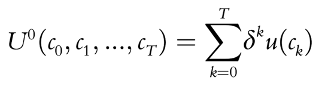
\includegraphics[width=0.8\linewidth]{Underinvestment1.png}
\end{figure}

\noindent where $0 < \delta < 1$, $c_i$ is consumption in the ith period, there are t more periods left in a person's life, and $u(c_k)$ is some function which transforms consumption in period k to utility. These consumption values must be bounded by the income one will have over the course of their life, which can be expressed mathematically as follows:
\begin{figure}[h]
    \centering
    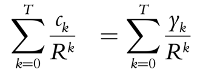
\includegraphics[width=0.5\linewidth]{underinvestment2.png}
\end{figure}

\noindent where $R^k$ is the gross per-period interest rate, $C_k$ is the consumption in period k, and $Y_k$ is the income in period k. Under this model, people will make their savings decisions by maximizing the utility function subject to the budget constraint, expressed mathematically below:
\begin{figure}[h]
    \centering
    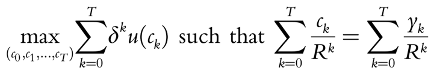
\includegraphics[width=1\linewidth]{underinvestment3.png}
\end{figure}

For the purpose of simplicity, the above model is one in which there is certainty about lifespan, future earnings, and interest rates. In my simulation I plan to include uncertainty about these values, although agents will have accurate beliefs about their likelihoods. Additionally, I will allow the interest rate on savings to be different from the interest rate on debt so as to be more reflective of the average person's experience. 

The key feature of the above model, for our purposes, is that people are necessarily time consistent. Time consistency means that if they plan in one period to save a certain amount in a subsequent period and their income predictions are correct, they will actually end up saving their planned amount when that subsequent period arrives. However, empirical evidence (and intuition) does not support the model’s prediction of time consistency, as will be examined in the prior work section. In an attempt to rectify this disparity between the model and reality, my simulation will include the concept of present bias. Present bias is the idea that people discount any period which is in the future by some constant amount in addition to the standard exponential discounting. This constant discounting is meant to account for the fact that people only ever exist in the present, and therefore overvalue it relative to anytime in the future, regardless of how far. Present bias modeled in this way can allow for time-inconsistent preferences.  

\subsection{Equity Premium Puzzle}
The equity premium puzzle is one of the most famous in economics. That returns on stocks are so much higher than on bonds constitutes a puzzle because this increased return should increase demand for stocks relative to bonds, lowering the difference between their returns. This is not to say that the existence of an equity premium is an anomaly under standard economics. Because stocks are riskier than bonds and people are assumed to be risk averse, defined as a preference for certain outcomes over uncertain outcomes with the same expected value, there must exist a positive equity premium. However, the magnitude of the premium should be reflective of the extent to which people are risk averse, and the historical magnitude of the premium implies a level of risk aversion far higher than anything within the generally accepted range within the literature. This will be explored further in the prior work section. 

The standard models predicts that people will make their decision of whether to enter the stock market at a given equity premium based on the expected utility of doing so compared to expected utility of purchasing bonds. Expected utility is the weighted average of the utilities of the various possible outcomes, weighted by the likelihood of those outcomes. Risk aversion comes into play because the utility function used to evaluate outcomes is not simply equal to their net gain or loss. Rather, it is some concave function over their wealth as a result of the net outcome. The concavity of the function implies risk aversion, because an increase in wealth will increase utility by a smaller amount that a decrease of the same size decreases it. Crucially, this model assumes that people pre-determine for how long they would hold a stock if they were to buy it and only consider the expected utility as calculated at the end of that period, with no consideration for its intervening fluctuations. 

In an attempt to explain the equity premium, my simulation will introduce two concepts from behavioral economics. They are loss aversion and bracketing. Loss aversion is the phenomena that people tend to perceive the pain of losing something to be about twice as large in magnitude to the positive emotion associated with gaining something of equivalent value. Loss aversion can help explain the equity premium because people are overweighting potential losses relative to potential gains, causing them to demand higher returns in order to take on risk. Bracketing, in this context, is the idea that people pay attention to the fluctuations of the market rather than to their net returns once they have sold the stock. This is relevant because the chance of having a loss in any given day, month, year, etc. is quite high, whereas the chance of having a net loss after tens of years is approximately zero. If people are also loss averse over the returns of these individual periods, it becomes clear how the returns they demand are much higher than those predicted by risk aversion alone.

\subsection{Violation of Efficient Market Hypothesis}
Underlying the efficient market hypothesis is the assumption that people form their beliefs about the fundamental value of a stock based on all publicly available information, and then accurately update that belief when they receive new information, whether that be in the form of price changes to the stock or new information about the company in question. To be accurate, a person must update their belief in accordance with Bayes rule, written out below:
\begin{figure}[H]
    \centering
    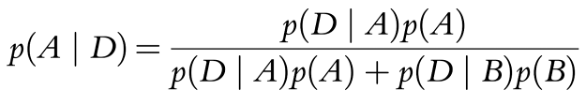
\includegraphics[width=1\linewidth]{EMH1.png}
\end{figure}

\noindent where A and B are the possible states of the world. Given some new information D, the above formula allows a person to accurately update their belief about the probability that A is the true state of the world. Under the assumption of universal Bayesian belief updating, the empirical observations (a)-(d), listed in the problem context section, are not possible. A possible explanation for these observations comes from the behavioral economics literature on non-standard belief updating, in particular the existence of extrapolative beliefs. Extrapolative beliefs are the result of an incorrect belief in the law of small numbers, which is the idea that a small sample will necessarily ‘look like’ the larger population from which it is drawn. Someone with extrapolative beliefs who sees that a stock has positive returns for multiple consecutive periods will therefore believe with too much confidence that the fundamental value of the stock is high. A portion of the population having such beliefs could plausibly explain the observations (a)-(d).

\subsection{Agent-Based Simulation}
Simulation is a technique which seeks to mimic a real-world process for the purpose of being able to manipulate parameters and see the effect of doing so. While a simulation relies upon a model of the world such as those previously discussed, it is more dynamic in that it has the advantage of being able to incorporate randomness over time and to apply the model to different agents who may have different characteristics and who can interact with each other. This project will primarily use agent-based simulation, a type of simulation which focuses on the characteristics and decisions of individuals and how the aggregation of those decisions creates the system we observe. In the words of Eric Bonabeau, a leader in the fields of complex systems and human decision-making, “ABM is a mindset more than a technology. The ABM mindset consists of describing a system from the perspective of its constituent units… [which] enables one to deal with more complex individual behavior, including learning and adaptation.”\cite{bonabeau}

\section{Prior Work}
This section will explore literature related to each of the three simulations, with two goals in doing so. The first is to examine past work that has been done to explain the anomaly and discuss how my project will complement this existing work. The second is to identify the sources from which relevant data and empirical estimates of parameters will be sourced, for the simulations for which this is needed.

\subsection{Underinvestment}
Much of the literature around low savings and investment rates focuses on structural barriers to these behaviors, such as increasing cost of living relative to wages and the disappearance of pensions. Still, the fact remains that people consistently report not saving as much for their retirement as they would like to be given their circumstances. A recent example of this comes from the TransAmerica center for Retirement Research’s annual report\cite{transamerica}, finding that 73\% of those 50 and older wished they had saved more on a consistent basis. Additionally, the report finds that nearly half of retirees decrease their consumption in retirement. Both of these figures contradict the standard model and point towards the need for explanations beyond structural challenges. Among the research in this area, present bias is a leading explanation. Goda et. al\cite{goda} find that an individual’s score on a questionnaire designed to detect present bias is correlated with their level of retirement savings. There has been work in integrating present bias into simulations of the life-cycle model, such as Peter Maxted’s work in estimating the welfare costs of present bias in the context of savings decisions.\cite{maxted} However, I am unaware of a simulation done explicitly to test for the existence of some value of loss aversion which aligns the standard model with empirical data.

This simulation in particular requires a significant amount of data in order to set up. Below is a list of the areas in which data is needed and a link to the reference for the location from which the data will be obtained:
\begin{enumerate}
    \item historical return on savings\cite{returns}
    \item historical interest rates on loans\cite{personalloan}
    \item death probability by age\cite{death}
    \item annual changes in income\cite{income}
    \item odds of unemployment\cite{unemployment}
    \item lump sum income\cite{inheritance}
    \item generally accepted range for the magnitude of present bias\cite{presentbias}
\end{enumerate}

\subsection{Equity Premium Puzzle}
The equity premium puzzle is a famous question within economics, and much has been written on its possible causes. In 1997, the influential behavioral economist Richard Thaler wrote a paper with colleague Jeremy Siegal in which they survey possible explanations and conclude that it is very difficult to explain the puzzle without some sort of irrationality of the type behavioral economics is focused on.\cite{thaler}  In 2007, Barberis and Huang were among the first to formalize the bracketing and loss aversion explanation of the equity premium puzzle, finding that the approach was promising and merited further research.\cite{BarberisEPP} The series of lotteries which I will use in order to model the stock market for the purpose of investigating the equity premium puzzle is a common way of modeling it within the behavioral economics literature. The sources of the data I will use to construct my model are listed below:
\begin{enumerate}
    \item historical equity premiums\cite{equitypremiums}
    \item utility function over wealth\cite{utilitywealth}
    \item empirical estimation of loss aversion coefficient\cite{lossaversion}
\end{enumerate}

\subsection{Violation of Efficient Market Hypothesis}
Violations of the efficient market hypothesis have been pointed out for nearly as long as the hypothesis itself has been around. References to the papers responsible for documenting the 4 observations I define as constituting violations of the hypothesis which I will attempt to resolve through the introduction of extrapolative beliefs are listed below. The idea of putting these 4 observations together and attempting to explain them simultaneously by using extrapolative beliefs is credited to Nicholas Barberis.\cite{BarberisEMH}
\begin{enumerate}
    \item medium term momentum\cite{MedTermMomentum}
    \item long term reversal\cite{LongTermReversal}
    \item excessive volatility\cite{volatility}
    \item bubbles\cite{bubbles}
\end{enumerate}

\section{Methods}
This section will discuss the setup of each of the three simulations. It will first include how the standard model will be set up and calibrated, and then how the relevant behavioral concept(s) will be included and calibrated, where relevant. In every case where the value of a parameter is drawn from some distribution, the distribution is determined by empirical work discussed in the above section. Similarly, the extent of any correlation between two variables will be determined by the literature discussed in the above section. 

\subsection{Underinvestment}
\subsubsection{Standard Setup and Calibration}
The simulation will be set up as series of periods, each representing a single year. 1000 agents will be created, each with a starting age of 22 and a starting income and wealth drawn randomly from a distribution. Starting income will be positively correlated with starting wealth. Each will have a utility function over life-cycle consumption, with a discount factor drawn randomly from a normal distribution. In every period other than the first, the following will be randomly drawn from a normal distribution for the simulation as a whole, with values correlated:
\begin{enumerate}
    \item return on savings
    \item interest rate on loans
\end{enumerate}
The following will be drawn from distributions for each agent, which are correlated with the agent’s current wealth, income, or age where applicable:
\begin{enumerate}
    \item percent change in income
    \item death
    \item employment status
    \item lump sum income
\end{enumerate}
\setenumerate
In each period, agents must make a choice of consumption and retirement status such that their expected lifetime utility is maximized subject to their expected budget constraint given their accurate beliefs as to probability and or magnitude of the various stochastic variables listed above, i.e. they know the properties of the distributions from which the values are drawn. For the sake of simplicity, all agents will begin receiving social security income at age 65. The simulation ends once the last agent has died.

The standard simulation will be calibrated by adjusting the distribution of discount factors such that the average ratio of yearly working-life consumption to yearly retirement consumption is equal to what people say via survey data they would like, discussed in the prior work section. 

\subsubsection{Introduction of Behavioral Factors}
Once the simulation has been calibrated such that it is empirically accurate given the assumption of time-consistent preferences, present bias will be introduced. Each agent will be given a present bias value drawn from a normal distribution, and the simulation will be run in the same way as it was before. The goal of this stage in the process is to see if there exists some distribution of present-bias values within a reasonable range such that the average ratio of yearly working-life to retirement consumption matches what is actually empirically observed. If so, this suggests that present bias is a plausible explanation for the underinvestment anomaly. 

\subsection{Equity Premium Puzzle}
\subsubsection{Standard Setup and Calibration}
To investigate the equity premium puzzle, I will model the choice of investing in the stocks or in bonds as a choice between choosing to take a series of 100 lotteries or not. In effect, this choice normalizes the return of bonds to zero, which is convenient in that it means the return from stocks is equal to the equity premium. Each lottery will represent a single month, and its payout in each month is drawn from a normal distribution. This approach to the Equity Premium Puzzle is different from the other two anomalies in that it is more of a math problem than a simulation and does not have multiple agents who interact with each other. The ‘simulation’ will be a calculation of whether a person would choose to take the series of lotteries or not, given that they are deciding based on the principle of expected utility, with a utility function over wealth determined empirically based on the literature in the prior work section. 

To calibrate the model such that it is consistent with the predictions of standard theory, the distribution of lottery outcomes will be manipulated such that it reaches the minimum level the person would be willing to accept. Whatever the average of this distribution is represents what the equity premium ‘should’ be. 

\subsubsection{Introduction of Behavioral Factors}
In the version of the model with behavioral factors, the average of the distribution of lottery outcomes will no longer be a dynamic value, and will instead be fixed at the historical average. Introducing the behavioral factors of bracketing and loss aversion presents a dilemma in that since there are two of them, there are an infinite number of value combinations which could result in the minimum risk profile such that the person accepts the series of lotteries. To resolve this, I will fix the value of loss aversion at 2, its average value within the literature, and only manipulate the bracket size to find its minimum value such that the person accepts the lottery series. I am choosing to fix loss aversion since literature estimating its value is more complete than that estimating the magnitude of bracketing. If there exists a bracket size within a reasonable range such that the person chooses to take the lottery series with an average payout of the historical equity premium magnitude, this suggests that the concepts of bracketing and loss aversion form a plausible explanation to the equity premium puzzle. 

\subsection{Violation of Efficient Market Hypothesis}
\subsubsection{Standard Setup}
For simplicity, this simulation will be over a singe asset. There will be 100 agents who are each assigned a valuation randomly from a normal distribution, representing their belief as to the fundamental value of the stock. Agents are not aware of where they fall within this distribution. Each agent is given an endowment of the stock, and for 15 periods they are free to trade, buying if their valuation is higher than the market price and selling if it is not. At an intermediate period, there will be some news related to the fundamental value of the stock, and agents will update their beliefs about their valuation in accordance with Bayes’ rule. Since all agents are Bayesian updaters, the trajectory of the stock price should not exhibit any of the characteristics (a)-(d). This simulation does not need to be calibrated because it is not designed to mimic any particular asset and does not rely on any parameters. 

\subsubsection{Introduction of Behavioral Factors}
In this stage, a portion of the 100 agents will be assigned to have extrapolative beliefs, meaning they will interpret the price change in response to the news relating to the value of the stock as more indicative of a change in fundamental value than it actually is. The Bayesian updating agents will be aware of the existence of extrapolative agents, meaning they will not have an incentive to immediately buy/sell in response to the price not being equal to fundamental value, preferring instead to wait until the peak/bottom of the overcorrection so as to make money off of it. The goal of this simulation will be to find if there exists a range of proportions of extrapolative updaters such that observations (a)-(d) occur within the model.

\section{Evaluation Metrics}
The quantifiable metrics for evaluating the success of each individual simulation have already been discussed in the previous section. In this section, I will argue that successful simulations as defined by these metrics constitute an effective argument in favor of the validity of behavioral economics concepts as true aspects of human nature whose inclusion improves economic frameworks. While the models upon which the simulations depend are vast oversimplifications given the complexities of the world, they are still effective at telling an intuitive and logically valid story about people’s motivations within a certain context. Given that both the models with and without behavioral considerations suffer from this same limitation, if the models with behavioral considerations do a better job of replicating reality the behavioral factors must be true aspects of human nature. Beyond supporting the validity of the ideas of behavioral economics, a successful version of this project would also support their increased inclusion in empirical research going forwards, as it would provide an example of them being successfully integrated with existing models and empirical data.

\section{Timeline}
Below are a list of milestones in the process of completing this project and the dates at which I would like to have them finished so as to stay on track:
\begin{enumerate}
    \item (end of May) Model 1: create distributions for each stochastic parameter based on historical data
    \item (end of June) Model 1: create and calibrate standard model
    \item (mid July) Model 1: introduce behavioral concepts and calibrate
    \item (end of August) Model 2: create and calibrate standard model
    \item (mid September) Model 2: introduce behavioral concepts and calibrate
    \item (mid October) Model 3: create standard model
    \item (mid November) Model 3: introduce behavioral concepts and calibrate
    \item (end November) Create visualizations of results
    \item (Mid December) Write final paper
\end{enumerate}

\printbibliography

\end{document}
    